\documentclass[10pt,sigconf]{acmart}

\settopmatter{printacmref=false, printccs=false, printfolios=false}

\usepackage{booktabs}
\usepackage[htt]{hyphenat}  % allow long \texttt{} tokens to break across lines
\usepackage{tikz}
\usetikzlibrary{arrows.meta,positioning,calc,fit,backgrounds,shapes.geometric,decorations.pathreplacing}

\graphicspath{{figure/}{figures/}}

\emergencystretch=1.5em  % absorb minor overfull lines in the narrow columns

% ---- Shared diagram palette (two-color accent) and node styles ----
\definecolor{cOn}{HTML}{1F6FB2}   % accent: on-chain Contract
\definecolor{cOnBg}{HTML}{E7F1F9}
\definecolor{cOff}{HTML}{C2570C}  % accent: off-chain Fisherman
\definecolor{cOffBg}{HTML}{FBEDE1}
\definecolor{cSup}{HTML}{6B7280}  % supporting services
\definecolor{cSupBg}{HTML}{F1F2F4}
\tikzset{
  rnode/.style={draw, rounded corners=2pt, align=center, font=\footnotesize,
    inner sep=4pt, minimum height=7mm},
  onchain/.style={rnode, draw=cOn, line width=0.6pt, fill=cOnBg, text=cOn!60!black},
  offchain/.style={rnode, draw=cOff, line width=0.6pt, fill=cOffBg, text=cOff!60!black},
  support/.style={rnode, draw=cSup, fill=cSupBg, text=cSup!30!black},
  ext/.style={rnode, draw=cSup, dashed, fill=white, text=cSup!30!black},
  state/.style={rnode, draw=cOn, fill=cOnBg, text=cOn!60!black, minimum width=15mm},
  term/.style={rnode, draw=cOff, fill=cOffBg, text=cOff!60!black, minimum width=15mm},
  flow/.style={-{Stealth[length=2mm]}, line width=0.5pt, font=\scriptsize},
  back/.style={flow, dashed, draw=cOff},
  life/.style={draw=cSup, line width=0.5pt},
}

% Formal statement environments: bold heading + italic statement (Walrus style)
\newtheoremstyle{reiythm}%
  {6pt}{6pt}%            space above / below
  {\itshape}%           body font (the statement, in italics)
  {0pt}%                indent
  {\bfseries}%          head font (bold "Definition N")
  {.}%                  punctuation after head
  {.5em}%               space after head
  {\thmname{#1}\thmnumber{ #2}\thmnote{ {\normalfont(#3)}}}% head: Name N (note)
\theoremstyle{reiythm}
\newtheorem{definition}{Definition}
\newtheorem{property}{Property}

\setcopyright{none}

\begin{document}

\title{Reiy Finance: Intent-based Meta DEX Aggregator}
\subtitle{v2.0 - June, 2026}

% ----------------------------------------------------------------
% Authors — add new \author blocks here as the team grows.
% Each block: \author{Name} \affiliation{\institution{}} \email{}
% ----------------------------------------------------------------
\author{Wyner Hoang}
\affiliation{\institution{Reiy Finance}\country{}}
\email{bach.hd.28@gmail.com}

\renewcommand{\shortauthors}{Wyner Hoang et al.}

\begin{abstract}
The DeFi ecosystem on Sui has matured into a full stack of decentralized
exchange models, spanning automated market makers, a native central limit
order book in DeepBook, and aggregators, all serving a large user base on a
platform built for parallel execution, low latency, and cheap fees. Yet
regardless of the model, liquidity remains fragmented across independent
protocols, and slippage stays an inherent cost that every venue tries to
minimize but cannot remove. At the same time, existing intent markets on other
ecosystems impose high entry costs on the agents that fill orders, which leads
to oligopoly and erodes the very execution quality that users should receive.

We present Reiy, the first intent based meta DEX aggregator on Sui. Rather than
selecting a pool or a route, a user submits an intent whose assets are escrowed
on chain, and a permissionless network of solvers competes in epoch gated
auctions to fill it at the best price by matching a coincidence of wants and by
sourcing external liquidity. Prevailing intent designs keep this coordination off
chain to preserve low latency and cost; Reiy instead escrows and enforces intents
on chain while retaining that profile, by confining the off chain coordinator to
selection and signing.

Reiy adapts the design of CoW Protocol to Sui through three contributions. First,
the SBBO admission floor reads an on chain reference price and rejects any intent
whose minimum falls below the market floor. Second, permissionless solver
competition removes the entry barriers that drive intent markets toward
oligopoly. Third, settlement exploits Sui Programmable Transaction Blocks and the
hot potato pattern to bind the off chain certificate to a single atomic on chain
transaction, so escrowed assets move only when every protection holds. Reiy
neither competes with nor replaces any venue on Sui; it is an execution layer that
turns the ecosystem's fragmented liquidity into depth a single trade can reach.
\end{abstract}

\maketitle

% ----------------------------------------------------------------
% Body
% ----------------------------------------------------------------

\section{Introduction}

\subsection{A Mature DeFi Stack on Sui}

Sui has grown into one of the most complete environments for decentralized
finance. Its object centric data model and parallel execution engine give
builders low latency settlement and cheap fees, and the ecosystem now offers a
full range of exchange primitives on top of this foundation
\cite{suidefistack}. Traders can route through automated market makers, post and
take on the native central limit order book in DeepBook, or rely on aggregators
that stitch these venues together. Lending, derivatives, and structured products
round out a stack that already serves a large and active user base.
% TODO(cite): Sui DeFi TVL milestone, e.g. DefiLlama Sui chain page and
% "Sui TVL Hits Record $2.6 Billion" (The Defiant, 2025) for a concrete figure.

Sui no longer lacks places to trade. What it lacks is a layer that turns this
breadth into a single efficient market rather than a set of isolated ones.

\subsection{Fragmentation and the Persistence of Slippage}

Every venue holds its own liquidity. An automated market maker, an order book,
and an aggregator each price the same pair against a different and partial view
of available depth, so capital that could clear a trade together sits divided
across protocols. A trader who wants the best outcome must compare venues, split
orders, and absorb the overhead of doing so manually.

Underneath this fragmentation lies a cost that no single venue can design away.
Slippage, the gap between a quoted price and the realized one, grows with trade
size and shrinks with available depth. Constant product pools price it directly
into their curve, and order books express it through limited depth at the top of
book. Every exchange tries to minimize slippage, yet none can remove it while
its liquidity stays siloed. The deeper the fragmentation, the worse the realized
price, and the more value leaks to arbitrage and reordering rather than to the
user.

\subsection{Why Existing Intent Markets Fall Short}

Intent based trading offers a way out. Rather than choosing a venue, a user
states what they want, such as a minimum amount to receive, and delegates
execution to agents who compete to satisfy it. CoW Protocol on Ethereum has
shown that this design can match opposing orders directly and aggregate external
liquidity to beat single venue execution \cite{documentationcowdaoe}.

The model is not without tension. A recent analysis of intent based markets
shows that the costs solvers must pay to participate restrict entry, and that
the resulting competition can collapse toward a small oligopoly
\cite{chitra2024analysisintentbasedmarkets}. When few agents compete, the
execution quality that intents promise to users erodes. Any intent system on a
new chain must therefore treat open and permissionless solver participation as a
first class design goal, not an afterthought. To date, no such system exists
natively on Sui, and designs built for Ethereum do not transfer cleanly to its
object centric model.

\subsection{Reiy}

Reiy, the first intent based meta DEX aggregator on Sui, adapts the design of CoW
Protocol \cite{documentationcowdaoe} to a chain whose fast finality and low fees
let the auction and settlement loop run at a cadence Ethereum cannot match. It is
deliberately not another DEX: rather than competing with the venues already on
Sui, it sits above them as an execution layer that turns their fragmented
liquidity into depth a single trade can reach.

The remainder of this paper develops the design. Section~2 fixes the preliminaries
and the research question, Section~3 the system model, and Section~4 the
architecture. Section~5 defines the core constructs: intents, the SBBO floor,
solvers, certificates, and the Programmable Transaction Block settlement that binds
them. Section~6 describes the off chain coordinator, Section~7 the economic model
and the REIY token, and Section~8 the resulting security properties.

% ================================================================
\section{Background and Preliminaries}
% ================================================================

This section introduces the primitives the rest of the paper relies on. Readers
familiar with Sui and intent based trading may skip ahead.

\subsection{The Sui Execution Model}

Sui organizes state as typed objects rather than as entries in a global account
map \cite{suidefistack}.
% TODO(cite): Sui whitepaper, https://docs.sui.io/paper/sui.pdf, for the object model.
An object is either owned by an address or shared, and a transaction declares
the objects it touches. Independent transactions then execute in parallel, which
gives Sui sub second finality and low fees. Two features matter for Reiy. First,
a \emph{shared object} can hold escrowed user assets that many parties may
interact with under rules the contract enforces. Second, a Programmable
Transaction Block (PTB) chains several Move calls into one atomic transaction,
and Move's linear \emph{hot potato} type lets a value created early in a PTB be
required to be consumed before the block ends. Together these let Reiy escrow
funds on chain and settle a whole batch in a single transaction that either
fully succeeds or fully reverts.

\subsection{Liquidity and the On-Chain Price Reference}

Sui hosts a full set of trading venues across automated market makers, order
books, and aggregators. Liquidity is partitioned across them, so a given pair is
priced against a different and partial view of total depth. Reiy depends on this
ecosystem in only one structural way: it reads a canonical on chain price. DeepBook,
the native central limit order book, exposes a per pool mid price that a contract
can query directly \cite{querypoolsui}, and Reiy uses this mid price as the
admission reference of Section~5. How a solver subsequently sources liquidity is
left entirely to the solver and is outside the protocol.

\subsection{Intents, Solvers, and Batch Auctions}

In an intent based market a user does not select a venue or a route. The user
signs an \emph{intent}, a statement of the desired outcome such as a minimum
amount to receive, and delegates execution to agents called \emph{solvers} that
compete to satisfy it \cite{documentationcowdaoe}. Aggregating intents into time
bounded \emph{batches} admits a coincidence of wants, in which opposing orders
clear against one another without price impact, and lets a solver source only the
residual externally.

In prevailing designs the intent and all coordination around it, including the
auction and the choice of solver, live off chain; only settlement touches the
chain. That off chain locus is what affords stable latency and low cost, since the
expensive coordination never pays for on chain execution. This frames Reiy's
central question: can an intent be escrowed and enforced on chain, making custody
and user protection trustless, while keeping the latency and cost of an off chain
market? Reiy answers yes, by escrowing the intent on chain and confining the off
chain coordinator to selection and signing.

A second tension concerns competition. A formal analysis of intent markets shows
that the cost of participating as a solver restricts entry and can drive the market
toward oligopoly, eroding the execution quality intents promise
\cite{chitra2024analysisintentbasedmarkets}. Reiy therefore treats permissionless
solver participation as a first class requirement, and Section~5 shows how on chain
verification makes it safe to admit any solver.

% ================================================================
\section{System Model}
% ================================================================

\subsection{Actors and Roles}

The protocol admits two sources of truth. The on chain \emph{Contract} is the
authority over custody and verification; the off chain \emph{Fisherman} is the
authority over coordination and certification. All other participants are
untrusted, and their claims are verified against one of these two authorities.
Table~\ref{tab:actors} states each role and its trust assumption.

\begin{table}[htbp]
  \centering
  \caption{Participants, roles, and trust assumptions.}
  \label{tab:actors}
  \begin{tabular}{@{}lp{3.6cm}l@{}}
    \toprule
    Participant & Role & Trust \\
    \midrule
    Trader & Originator of an escrowed intent & Untrusted \\
    Solver & Bonded execution agent & Untrusted \\
    Fisherman & Off chain coordinator and certifier & Bounded \\
    Contract & On chain custody and verification authority & Trusted \\
    \bottomrule
  \end{tabular}
\end{table}

The Contract is the source of truth for state and safety: it admits intents,
verifies the certificate, and enforces the payout floors and the atomicity of
settlement. The Fisherman is the source of truth for ordering and selection; it
is the sole off chain coordinator and subsumes the auctioneer, keeper, and relayer
roles of earlier designs. The DeepBook mid price is consumed as a verification
input, not as a trusted party.

\subsection{Trust and Threat Model}

Reiy is trust minimized rather than trustless. The Contract is trusted as the
on chain rule enforcer; the Fisherman is trusted only for liveness, its authority
bounded by what the Contract accepts; traders, solvers, and external liquidity are
untrusted and verified on chain. A malicious or offline Fisherman can therefore
stall progress but never cause loss of funds, since custody and every user
protection live in the Contract; Section~8 states the resulting guarantees
formally.

The remaining adversaries reduce to this separation. Solver collusion is countered
by permissionless entry, since any outside party can undercut a colluding group;
manipulation of the reference price is bounded by restricting trading to supported
pairs and validating the price at read time; a winning solver that fails to settle
is penalized by bond slashing and superseded through fallback.

\subsection{Design Goals and Properties}

Reiy is built to guarantee the following properties, each established by the
mechanism in later sections.

\begin{itemize}
  \item \textbf{Non custodial.} Escrow lives in the Contract and off chain
    authority is bounded, so user funds are never under a coordinator's control.
  \item \textbf{User protected execution.} An SBBO admission floor and a per
    intent protected minimum are enforced on chain, and they hold even after
    fees are deducted.
  \item \textbf{Atomic settlement.} A batch settles in one PTB through the hot
    potato pattern, so it either completes fully or reverts.
  \item \textbf{Permissionless solver competition.} Any bonded party may solve,
    with no whitelist, which directly answers the oligopoly risk of intent
    markets \cite{chitra2024analysisintentbasedmarkets}.
  \item \textbf{Liveness and no stuck funds.} Epoch advance and fallback are
    permissionless, so no party can freeze the protocol.
  \item \textbf{Verifiable and auditable.} Events expose committed and actual
    values so indexers and auditors can reconstruct the quality of every batch.
\end{itemize}

% ================================================================
\section{System Overview}
% ================================================================

\subsection{Architecture}

Reiy is split between an on chain core and an off chain coordinator, the two
sources of truth of Section~3, surrounded by supporting services that hold no
authority. The Contract escrows intents, verifies certificates, and enforces the
floors and fees. The Fisherman groups intents, runs the auction, and signs
certificates. Around them, an Indexer decodes on chain events into queryable
state and an OrderBook API serves quotes and open intents to solvers. None of
these supporting services can move funds or override a protection; the system's
guarantees never depend on them.

\begin{figure*}[htbp]
  \centering
  \resizebox{\textwidth}{!}{%
  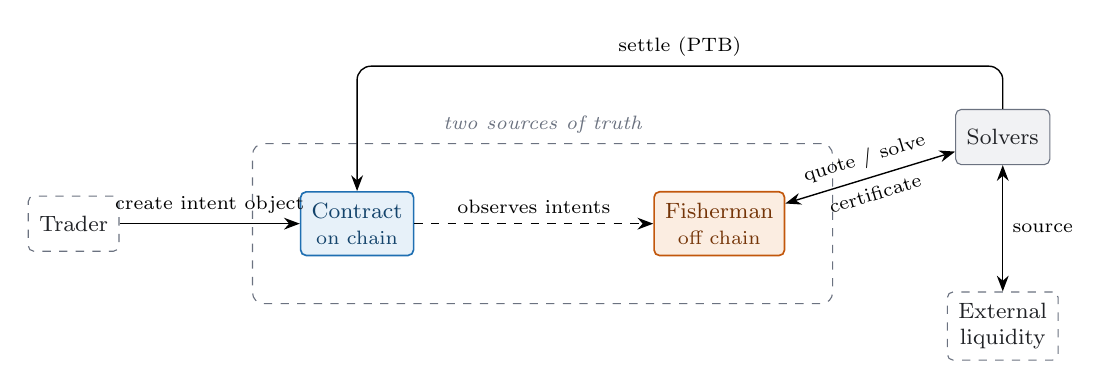
\begin{tikzpicture}[font=\scriptsize, >={Stealth[length=2mm]},
      e/.style={draw, line width=0.5pt}]
    % --- nodes, explicit coordinates ---
    \node[ext]      (trader)   at (0,0)      {Trader};
    \node[onchain]  (contract) at (3.6,0)    {Contract\\\scriptsize on chain};
    \node[offchain] (fisher)   at (8.2,0)    {Fisherman\\\scriptsize off chain};
    \node[support]  (solvers)  at (11.8,1.1) {Solvers};
    \node[ext]      (liq)      at (11.8,-1.3) {External\\liquidity};
    % --- two-sources-of-truth frame ---
    \begin{scope}[on background layer]
      \node[draw=cSup, dashed, rounded corners, inner sep=6mm,
        fit=(contract)(fisher),
        label={[font=\scriptsize\itshape, cSup]above:two sources of truth}] (frame) {};
    \end{scope}
    % --- main flow ---
    \draw[e,->] (trader) -- node[above]{create intent object} (contract);
    \draw[e,->,dashed] (contract) -- node[above]{observes intents} (fisher);
    \draw[e,<->] (fisher) -- node[above, sloped]{quote / solve}
                                node[below, sloped]{certificate} (solvers);
    \draw[e,<->] (solvers) -- node[right]{source} (liq);
    % settle routed over the top, clear of every node
    \draw[e,->, rounded corners=5pt]
      (solvers.north) -- (11.8,2.0) -- node[above]{settle (PTB)}
      (3.6,2.0) -- (contract.north);
  \end{tikzpicture}}
  \caption{The main flow between the two sources of truth.}
  \label{fig:architecture}
\end{figure*}

\subsection{Intent Lifecycle}

A trade moves through one epoch as the sequence of Figure~\ref{fig:lifecycle}.
The Contract keeps the design small, escrowing intents, verifying certificates,
and settling without any on chain phase machine; the phase sequencing itself is
orchestrated off chain by the Fisherman. Intents are collected behind their SBBO
floors, solvers build settlement plans over the batch, the Fisherman ranks the
valid ones and certifies a winner, and that winner settles the certified plan in a
single PTB. Section~5 defines each step. If no valid solution arrives or the winner
fails to settle in time, a permissionless fallback advances the epoch and returns
the affected intents to the next batch, so the protocol never stalls.

\begin{figure}[htbp]
  \centering
  \resizebox{\columnwidth}{!}{%
  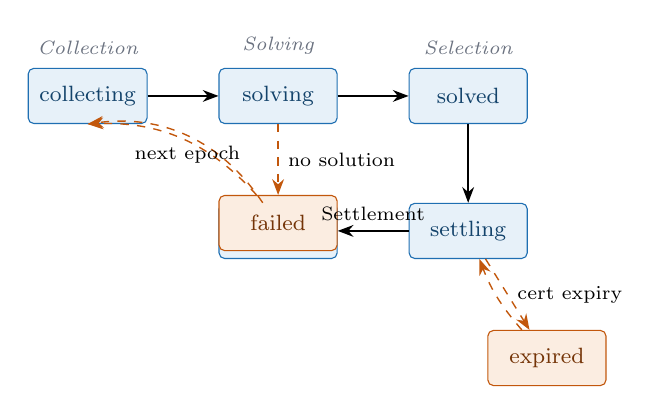
\begin{tikzpicture}[node distance=7mm and 9mm]
    \node[state] (col) {collecting};
    \node[state, right=of col] (solv) {solving};
    \node[state, right=of solv] (sold) {solved};
    \node[state, below=10mm of sold] (settling) {settling};
    \node[state, left=of settling] (settled) {settled};
    \node[term, below=9mm of solv] (failed) {failed};
    \node[term, below=9mm of settling, xshift=10mm] (expired) {expired};
    % phase captions under the happy path
    \node[font=\scriptsize\itshape, cSup, above=0.5mm of col] {Collection};
    \node[font=\scriptsize\itshape, cSup, above=0.5mm of solv] {Solving};
    \node[font=\scriptsize\itshape, cSup, above=0.5mm of sold] {Selection};
    % happy path
    \draw[flow] (col) -- (solv);
    \draw[flow] (solv) -- (sold);
    \draw[flow] (sold) -- (settling);
    \draw[flow] (settling) -- node[above, font=\scriptsize]{Settlement} (settled);
    % fallback edges
    \draw[back] (solv) -- node[right, font=\scriptsize]{no solution} (failed);
    \draw[back] (settling) -- node[right, font=\scriptsize]{cert expiry} (expired);
    \draw[back] (failed) to[bend right=25] (col.south);
    \draw[back] (expired) to[bend left=10] (settling);
    \draw[back] (settled) to[bend right=32] node[below, font=\scriptsize]{next epoch} (col.south);
  \end{tikzpicture}}
  \caption{Per epoch intent lifecycle (Fisherman round states; settled and the
    dashed paths return intents to the next epoch).}
  \label{fig:lifecycle}
\end{figure}

\subsection{Where Each Guarantee Lives}

Each design goal of Section~3.3 maps to a point in this lifecycle: the SBBO floor
protects users at admission (Section~5.2), permissionless competition and ranking
occur while solving and selecting (Section~5.3), and certificate verified atomic
settlement enforces the protected minimums (Sections~5.4 and~5.5). The economic
model of Section~7 aligns incentives without touching protected funds.

% ================================================================
\section{Protocol Design}
% ================================================================

The protocol is built from five core constructs: the \emph{intent}, the
\emph{SBBO floor}, the \emph{solver}, the \emph{certificate}, and the
\emph{settlement transaction}. We define each in turn and then describe epoch
progression. The construct names and parameters follow the Move implementation.

\subsection{Intents}

\begin{definition}[Intent]
An intent is a shared object \texttt{Intent<Sell, Buy>} that escrows a trader's
sell asset together with the terms under which it may be filled.
\end{definition}

\noindent It records the locked \texttt{sell\_balance}, the effective \texttt{min\_amount\_out},
the SBBO floor and reference mid price fixed at admission, the slippage tolerance,
a partial fill flag, a target epoch, and a deadline; it also retains the original
sell amount and minimum so that proportional minimums remain comparable across
partial fills. Escrow is non custodial: until settlement or cancellation the
asset remains in the object, and only its owner may cancel, recovering the full
balance.

An intent is created through the auction module, which reads the DeepBook mid
price \cite{querypoolsui}, computes the SBBO floor, verifies that the pair is
supported and that the slippage tolerance is within the configured maximum, and
admits the intent only if its minimum clears the floor.

\subsection{The SBBO Floor}

\begin{definition}[SBBO floor]
The SBBO floor, for Sui Best Bid and Offer, is the on chain lower bound that an
intent's minimum must clear at admission, derived from the live market price so
that no intent can be admitted with an unreasonably low minimum.
\end{definition}

\noindent Let $x$ be the sell amount, $P$ the DeepBook mid price
\cite{querypoolsui} scaled by $10^9$, and $\sigma$ the slippage tolerance in basis
points. The expected output is taken in the pool's direction,
\[
  \mathit{out} =
  \begin{cases}
    \lfloor x \cdot P / 10^9 \rfloor & \text{selling base for quote,}\\[2pt]
    \lfloor x \cdot 10^9 / P \rfloor & \text{selling quote for base,}
  \end{cases}
\]
and the admission floor applies the tolerance,
\[
  F = \left\lceil \mathit{out} \cdot \frac{10{,}000 - \sigma}{10{,}000} \right\rceil .
\]
An intent is admitted only if $\texttt{min\_amount\_out} \ge F$. The tolerance is
bounded by a configurable maximum, by default 500 basis points with a hard ceiling
of 2{,}000 basis points, and the mid price must exceed a configured minimum or the
read aborts. Because $F$ is computed from a live on chain reference and stored on
the object, neither the solver nor the coordinator can later admit a fill that
ignores the market.

\subsection{Solvers}

\begin{definition}[Solver]
A solver is an untrusted, bonded agent that proposes how a batch of intents should
be filled, competing permissionlessly to have its proposal selected.
\end{definition}

\noindent Participation is open: any party posting the minimum bond of Section~7
may compete, and the protocol places no constraint on how a solver obtains
liquidity. A solver may clear opposing intents against one another
as a coincidence of wants, which carries no price impact, and source any residual
externally; these strategies are economic choices internal to the solver and
outside the protocol.

A solver expresses its proposal as a \emph{solution}: per intent, a fill amount, a
gross payout, and the protected minimum it commits to, together with a single
\emph{score} that measures the solution's total quality in one comparable unit. A
solution is valid only if its epoch matches the batch, its per intent vectors are
well formed and unexpired, and each entry satisfies
\[
  \mathit{gross\ payout} \ge \mathit{protected\ min} \ge \mathit{user\ minimum},
\]
with a positive fill not exceeding the intent's remaining amount. Valid solutions
are ranked by score and the highest wins, ties broken deterministically. Because
admission is permissionless and ranking depends only on score, any outside solver
can win by offering strictly better execution, which is the structural
countermeasure to the entry barriers that drive intent markets toward oligopoly
\cite{chitra2024analysisintentbasedmarkets}.

\subsection{Certificates}

\begin{definition}[Certificate]
A certificate is the off chain coordinator's signed authorization of a specific
settlement, and the sole credential that lets a solver act on escrowed funds.
\end{definition}

\noindent The Fisherman signs a \texttt{SolutionMessage} with its Ed25519 key,
binding the protocol state and config object identifiers, the key version, the
epoch, the solver address, the traded types, and the per intent fills, gross
payouts, and protected minimums, together with an expiry. The certificate carries
no authority of its own; it is meaningful only because the Contract reconstructs
the same message from on chain state and verifies the signature, so the
coordinator can authorize a plan but cannot alter the rules that bind it.

\subsection{Settlement via Programmable Transaction Blocks}

\begin{definition}[Settlement]
A settlement is the single Programmable Transaction Block (PTB) in which the
winning solver redeems a certificate, releasing escrow and delivering the
certified payouts atomically.
\end{definition}

\noindent Settlement is where the certified plan meets on chain enforcement, and
where Reiy exploits the structure of Sui transactions. The winning solver executes
the whole batch in one PTB (Figure~\ref{fig:settle}), so verification, the release
of escrow, and the delivery of payouts all commit or all revert.

Two properties of the Sui execution model make this possible. A PTB composes
several Move calls into one transaction and passes the typed result of one call as
the input to the next, so a value produced by verification can be threaded into
the calls that release escrow and deliver payouts without ever leaving the
transaction. The \emph{hot potato} pattern then makes that threading mandatory. A
Move value whose type has none of the \texttt{copy}, \texttt{drop}, \texttt{store},
or \texttt{key} abilities cannot be copied, discarded, or stored; it can only be
unpacked by a function in its defining module. A value of such a type created in
the middle of a PTB therefore obligates a later call in the same PTB to consume
it, or the transaction is not well formed and cannot execute. Reiy uses this to
turn a procedural settlement into a guarantee enforced by the type system rather
than by trust.

Concretely, \texttt{take\_authorized\_intent} returns the escrowed sell coin
together with a \texttt{SettlementReceipt} that has no abilities, a true hot
potato. The receipt records the intent and its certified payout, and the only
function that can consume it is \texttt{settle\_intent}. The instant a solver
takes an intent's escrow it holds a receipt it cannot drop, store, or pass
outside the transaction, so it is compelled to call \texttt{settle\_intent} and
deliver the exact certified payout within the same PTB. There is no path in which
escrow leaves the contract without a matching settlement, and the property holds
for every intent in the batch at once.

\begin{figure}[htbp]
  \centering
  \resizebox{\columnwidth}{!}{%
  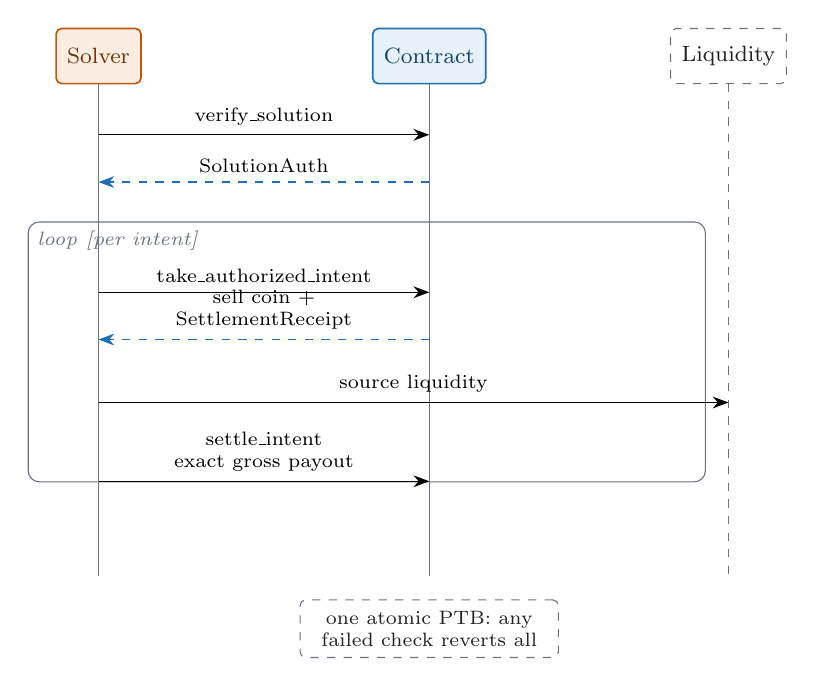
\begin{tikzpicture}
    % --- lifelines ---
    \node[offchain] (s) at (0,0) {Solver};
    \node[onchain] (c) at (4.2,0) {Contract};
    \node[ext] (l) at (8,0) {Liquidity};
    \def\ytop{-0.7} \def\ybot{-6.6}
    \draw[life] (s) -- (0,\ybot);
    \draw[life] (c) -- (4.2,\ybot);
    \draw[life, dashed] (l) -- (8,\ybot);
    % --- messages ---
    \draw[flow] (0,-1.0) -- node[above]{verify\_solution} (4.2,-1.0);
    \draw[flow, dashed, draw=cOn] (4.2,-1.6) -- node[above]{SolutionAuth} (0,-1.6);
    % loop frame
    \node[draw=cSup, rounded corners, inner sep=2mm, minimum width=86mm,
      minimum height=33mm, anchor=north west, font=\scriptsize\itshape, cSup,
      label={[anchor=north west, font=\scriptsize\itshape, cSup]north west:loop [per intent]}]
      (loop) at (-0.9,-2.1) {};
    \draw[flow] (0,-3.0) -- node[above]{take\_authorized\_intent} (4.2,-3.0);
    \draw[flow, dashed, draw=cOn] (4.2,-3.6) -- node[above, align=center]{sell coin +\\SettlementReceipt} (0,-3.6);
    \draw[flow] (0,-4.4) -- node[above]{source liquidity} (8,-4.4);
    \draw[flow] (0,-5.4) -- node[above, align=center]{settle\_intent\\\scriptsize exact gross payout} (4.2,-5.4);
    % atomic note
    \node[ext, anchor=north, text width=30mm, font=\scriptsize] at (4.2,-6.9)
      {one atomic PTB: any failed check reverts all};
  \end{tikzpicture}}
  \caption{The single PTB settlement sequence.}
  \label{fig:settle}
\end{figure}

Three checks make this safe. First, \texttt{verify\_solution} rebuilds the message
from on chain state, so the epoch, object ids, and token types cannot be forged,
and it checks the sender is the named solver, the certificate has not expired, and
the Ed25519 signature matches the configured coordinator key. It returns a
\texttt{SolutionAuth} that fixes the exact list of intents and payouts.

Second, each \texttt{take\_authorized\_intent} call advances through the certified
list in order, and requires that the intent id matches the next entry, that the
intent's \texttt{target\_epoch} equals the certificate epoch, that it has not
expired or already been partially filled this epoch, and that the committed
\texttt{protected\_min} is at least the intent's own minimum. It returns the
escrowed sell coin and the \texttt{SettlementReceipt} hot potato described above,
which obligates the matching \texttt{settle\_intent} call.

Third, \texttt{settle\_intent} requires the delivered buy coin to equal the
certified gross payout exactly, confirms the solver is active and bonded, deducts
fees so the net stays at or above the protected minimum, and transfers the net to
the trader. Any failed check reverts the whole PTB, so the trader's floor holds
even after fees.

\subsection{Epochs and Partial Fills}

The on chain state keeps only an epoch counter, a start timestamp, the set of
intents partially filled this epoch, and fee aggregates. There is no on chain
phase machine; epoch progression is permissionless. Anyone may call
\texttt{advance\_epoch} once the minimum collection time has passed, which
increments the epoch and clears the partial fill set, so the protocol cannot be
frozen by a stalled coordinator.

A partial fill consumes part of an intent and rolls the remainder forward. The
proportional minimum for a fill of size $f$ on an intent with original sell amount
$x_0$ and original minimum $m_0$ is
\[
  m_{\mathit{eff}} = \left\lceil m_0 \cdot f / x_0 \right\rceil ,
\]
computed against the original amounts so that successive partials stay comparable.
The residual advances its \texttt{target\_epoch} by one and re enters the next
batch, and the contract forbids two fills of the same intent within one epoch.

% ================================================================
\section{The Fisherman Coordinator}
% ================================================================

The Fisherman is the off chain source of truth for coordination. It holds no user
funds and cannot override any on chain check; it exists to make solver competition
fast and to produce the certificates the contract verifies.

\subsection{Services}

The coordinator is organized as a small set of services. An Indexer ingests the
Reiy contract events from Sui, and an Orderbook exposes the open intents drawn
from that index. A Quote service fans pre trade quote requests to enabled solvers
and ranks the replies. An Auction service groups open intents into rounds by token
pair and epoch. A Driver calls solver endpoints with bounded timeouts, a Scoring
service validates and ranks the responses, and a Certificate service signs the
canonical settlement message. A Settlement watcher marks expired certificates so a
round can be retried.

\subsection{Pre-Trade Quotes}

Before committing an intent, a trader may request an indicative quote. The
Fisherman normalizes the request and fans it to every enabled solver in parallel,
collects the replies within a bounded window, discards the late or invalid ones,
and returns the best valid quote, as shown in Figure~\ref{fig:quote}. The flow is
purely informational: it touches no escrow and binds no party, and the trader
proceeds to create an intent only if the quote is acceptable.

\begin{figure}[htbp]
  \centering
  \resizebox{\columnwidth}{!}{%
  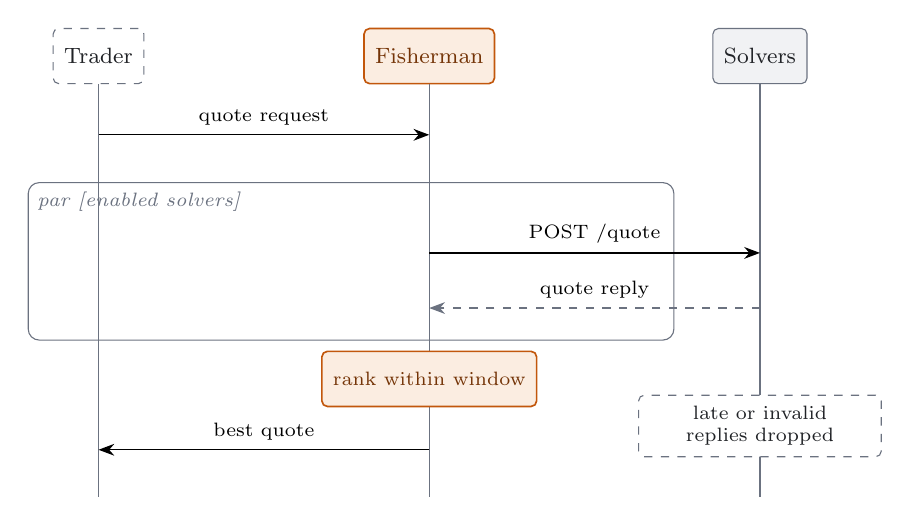
\begin{tikzpicture}
    % --- lifelines ---
    \node[ext]      (t) at (0,0)   {Trader};
    \node[offchain] (f) at (4.2,0) {Fisherman};
    \node[support]  (s) at (8.4,0) {Solvers};
    \def\ybot{-5.6}
    \draw[life] (t) -- (0,\ybot);
    \draw[life] (f) -- (4.2,\ybot);
    \draw[life] (s) -- (8.4,\ybot);
    % --- messages ---
    \draw[flow] (0,-1.0) -- node[above]{quote request} (4.2,-1.0);
    % fan-out frame
    \node[draw=cSup, rounded corners, inner sep=2mm, minimum width=82mm,
      minimum height=20mm, anchor=north west, font=\scriptsize\itshape, cSup,
      label={[anchor=north west, font=\scriptsize\itshape, cSup]north west:par [enabled solvers]}]
      (par) at (-0.9,-1.6) {};
    \draw[flow] (4.2,-2.5) -- node[above]{POST /quote} (8.4,-2.5);
    \draw[flow, dashed, draw=cSup] (8.4,-3.2) -- node[above]{quote reply} (4.2,-3.2);
    % rank activation on Fisherman lifeline
    \node[offchain, minimum width=24mm, font=\scriptsize] at (4.2,-4.1)
      {rank within window};
    \draw[flow] (4.2,-5.0) -- node[above]{best quote} (0,-5.0);
    \node[ext, anchor=north, text width=28mm, font=\scriptsize] at (8.4,-4.3)
      {late or invalid replies dropped};
  \end{tikzpicture}}
  \caption{Pre-trade quote flow: the Fisherman fans a request to enabled solvers
    in parallel and returns the best valid reply.}
  \label{fig:quote}
\end{figure}

\subsection{Round and Certificate Lifecycle}

A round moves through the states \texttt{collecting}, \texttt{solving},
\texttt{solved}, \texttt{settling}, and \texttt{settled}, with \texttt{expired}
and \texttt{failed} for the unhappy paths. Open intents are grouped into a
collecting round, defaulting to four intents per round and never more than ten.
Once the collection window passes, the round moves to solving, enabled solvers are
asked to solve, and the highest scoring valid plan is selected. The Certificate
service then signs the solution, and when the winning plan carries a Coincidence
of Wants counter leg it signs both legs as a pair. The certificate itself runs
\texttt{issued}, \texttt{settling}, \texttt{settled}, and is marked
\texttt{expired} or \texttt{reissued} if the winner does not settle in time. An
administrator endpoint reissues a certificate to the next candidate, and because
on chain settlement is always available for a live epoch, a fresh certificate can
settle immediately.

\subsection{API Surface}

The external interface follows the Coincidence of Wants convention with
\texttt{/quote}, \texttt{/solve}, \texttt{/reveal}, \texttt{/settle}, and
\texttt{/notify}, while the wire model is Sui native, carrying object ids, Move
type names, fills, protected minimums, and certificate expiry. Read endpoints
expose the orderbook, active auctions, and signed certificates, and an event
stream lets integrators follow rounds without speaking to the indexer directly.
Quote collection is bounded by a short window, by default a little over a second,
and replies that miss it are reported as failed rather than allowed to stall the
round.

% ================================================================
\section{Economic Model}
% ================================================================

The economic model has three layers: the fee the protocol charges, the revenue
model that fee produces, and the REIY token that secures and rewards the network.
We present the mainnet design; the current testnet contracts use a simpler in kind
fee split and a SUI bond, which mainnet supersedes.

\subsection{Fee Structure}

Reiy charges a fee only on a settled intent, taken from the gross payout and
structured so the trader's net never falls below the protected minimum. The fee
has two components. A \emph{base fee} is a flat rate on the notional, set at
0.02\% by default and 0.01\% for correlated or stable pairs; it ensures the
protocol earns a small, predictable amount on every trade even when competition
drives surplus to zero. A \emph{surplus fee} then takes a share, 20\% by default,
of the surplus delivered above the user's protected minimum, capped at 0.15\% of
notional. The total is capped at 0.25\% of notional, so the net payout always
remains at or above the protected minimum.

\begin{table}[htbp]
  \centering
  \caption{Fee parameters (governable initial values).}
  \label{tab:fees}
  \begin{tabular}{@{}lll@{}}
    \toprule
    Parameter & Default & Basis \\
    \midrule
    Base fee (standard) & 0.02\% & of notional \\
    Base fee (correlated) & 0.01\% & of notional \\
    Surplus fee & 20\% & of surplus \\
    Surplus fee cap & 0.15\% & of notional \\
    Total fee cap & 0.25\% & of notional \\
    \bottomrule
  \end{tabular}
\end{table}

Figure~\ref{fig:fee} shows how a settled payout is partitioned. The base and
surplus fees accrue to a per asset protocol treasury, denominated in the traded
asset. The solver is rewarded separately, in REIY rather than from the fee, and
additionally retains any execution margin it captures above the certified payout.
Tying the surplus fee to delivered surplus makes the protocol's revenue grow
precisely when users are filled better than their floor, never at their expense.

\begin{figure}[htbp]
  \centering
  \resizebox{\columnwidth}{!}{%
  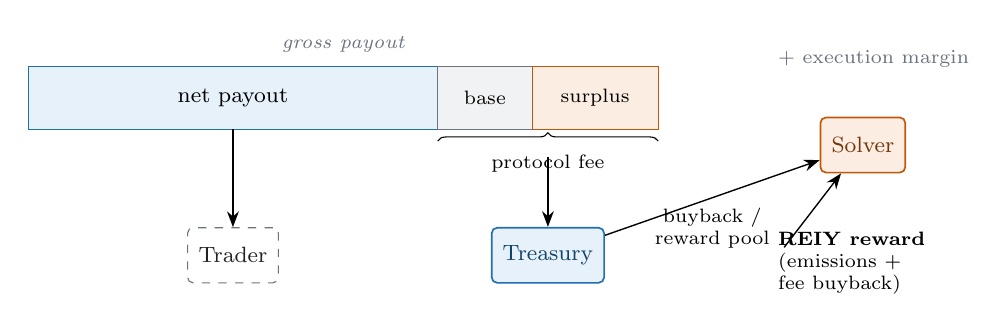
\begin{tikzpicture}[font=\footnotesize]
    % gross payout bar split into net | base | surplus fee
    \fill[cOnBg, draw=cOn] (0,0) rectangle (5.2,0.8);
    \fill[cSupBg, draw=cSup] (5.2,0) rectangle (6.4,0.8);
    \fill[cOffBg, draw=cOff] (6.4,0) rectangle (8.0,0.8);
    \node at (2.6,0.4) {net payout};
    \node[font=\scriptsize] at (5.8,0.4) {base};
    \node[font=\scriptsize] at (7.2,0.4) {surplus};
    \node[anchor=south, font=\scriptsize\itshape, cSup] at (4.0,0.85) {gross payout};
    \draw[decorate, decoration={brace, amplitude=3pt}] (5.2,-0.15) -- (8.0,-0.15);
    \node[anchor=north, font=\scriptsize] at (6.6,-0.2) {protocol fee};
    % recipients
    \node[ext] (user) at (2.6,-1.6) {Trader};
    \node[onchain] (treasury) at (6.6,-1.6) {Treasury};
    \node[offchain] (solver) at (10.6,-0.2) {Solver};
    \draw[flow] (2.6,0) -- (user);
    \draw[flow] (6.6,-0.35) -- (treasury);
    \draw[flow] (treasury) -- node[below, font=\scriptsize, align=center]{buyback /\\reward pool} (solver);
    \node[anchor=west, font=\scriptsize, align=left] at (9.4,-1.7)
      {{\bfseries REIY reward}\\(emissions +\\fee buyback)};
    \draw[flow] (9.6,-1.5) -- (solver);
    \node[anchor=west, font=\scriptsize, align=left, cSup] at (9.4,0.9)
      {+ execution margin};
  \end{tikzpicture}}
  \caption{Settlement payout split: the trader keeps the net, the protocol fee
    funds the treasury, and the solver is rewarded in REIY plus any execution
    margin.}
  \label{fig:fee}
\end{figure}

\subsection{Business Model}

Reiy sells execution quality. Its product is the surplus that a competitive solver
network delivers over what a trader would obtain unaided, and the protocol
monetizes a slice of that surplus rather than the trader's principal. Since the
total fee is bounded so the net stays at or above the protected minimum
(Section~7.1), every unit of revenue is drawn from value the network created,
never from the amount the user was guaranteed. The business is positive sum: Reiy
earns only when it makes a trader better off.

Revenue arrives in two streams that hedge one another. The \emph{base fee} is a
thin, volume linked charge that scales with settled value and yields a predictable
floor even when solver competition compresses surplus toward zero. The
\emph{surplus fee} is a value linked charge that scales with the price improvement
actually delivered, and is largest exactly when execution quality is highest. In a
maturing market the two move in opposite directions: sharper competition erodes per
trade surplus but attracts more flow, so the base fee floor grows as the surplus
fee thins. Revenue therefore does not collapse in the very equilibrium that best
serves users.

The unit economics are favorable. Revenue per trade is capped at 0.25\% of notional
and in practice sits well below that, while the protocol's marginal cost to settle
a trade is close to zero: the winning solver pays settlement gas, and the off chain
coordinator is a fixed cost that does not grow with volume. Gross margin per settled
trade is thus high, and the protocol's real cost base is not settlement but the
incentive it pays to keep the solver side competitive.

That incentive is paid in REIY rather than out of the fee, which lets early growth
run ahead of revenue. Solvers earn REIY on top of the execution margin they already
capture, so the network can bootstrap a deep, competitive solver set through
scheduled emissions before fee revenue is material. As volume grows, the treasury,
which accrues fees in the traded assets, funds the REIY buyback that replenishes the
reward pool, so emissions taper and real revenue takes over the cost of incentives.
The crossover, where fee funded buyback covers the rewards needed to retain solvers,
marks the transition from a subsidized network to a self funding one
(Figure~\ref{fig:crossover}).

\begin{figure}[htbp]
  \centering
  \resizebox{0.92\columnwidth}{!}{%
  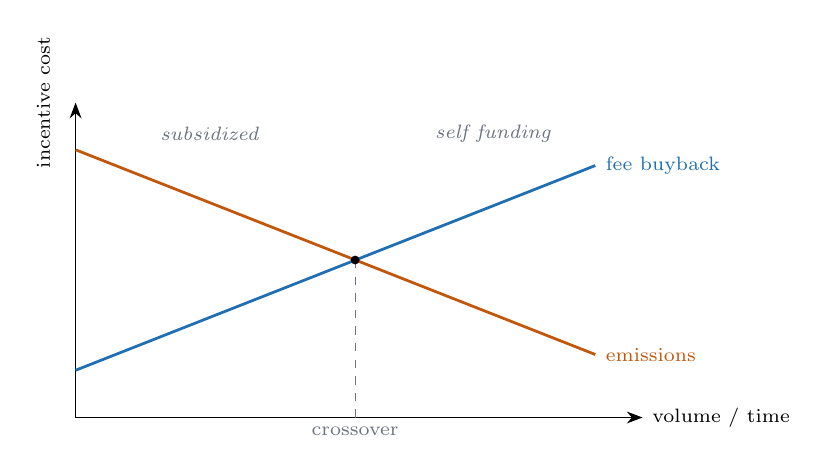
\begin{tikzpicture}[font=\footnotesize, >={Stealth[length=2mm]}]
    % axes
    \draw[->, line width=0.5pt] (0,0) -- (7.2,0) node[right, font=\scriptsize]{volume / time};
    \draw[->, line width=0.5pt] (0,0) -- (0,4) node[left, font=\scriptsize, rotate=90, anchor=south, yshift=2mm]{incentive cost};
    % emissions: high to low ; buyback: low to high (straight lines cross at ~(3.55,2.0))
    \draw[cOff, line width=1pt] (0,3.4) -- (6.6,0.8) node[right, font=\scriptsize, cOff]{emissions};
    \draw[cOn, line width=1pt] (0,0.6) -- (6.6,3.2) node[right, font=\scriptsize, cOn]{fee buyback};
    % crossover
    \coordinate (X) at (3.55,2.0);
    \draw[dashed, cSup] (X) -- (3.55,0) node[below, font=\scriptsize]{crossover};
    \fill (X) circle (1.6pt);
    \node[font=\scriptsize\itshape, cSup] at (1.7,3.6) {subsidized};
    \node[font=\scriptsize\itshape, cSup] at (5.3,3.6) {self funding};
  \end{tikzpicture}}
  \caption{Bootstrap to self funding. Scheduled emissions fund solver rewards early;
    fee funded buyback overtakes them at the crossover, after which real revenue
    sustains incentives.}
  \label{fig:crossover}
\end{figure}

Value compounds through a clear loop (Figure~\ref{fig:flywheel}). Better execution
attracts flow, flow produces fees, fees fill the treasury, the treasury funds
rewards and buyback, and deeper rewards draw more solvers whose competition improves
execution again. The REIY token captures this loop: its value is underpinned by fee
funded buyback, its circulating supply is reduced by the bonds solvers must lock, and
its holders govern the parameters that tune the system. A treasury denominated in
real traded assets backs the token, rather than the token backing the protocol.

\begin{figure}[htbp]
  \centering
  \resizebox{0.82\columnwidth}{!}{%
  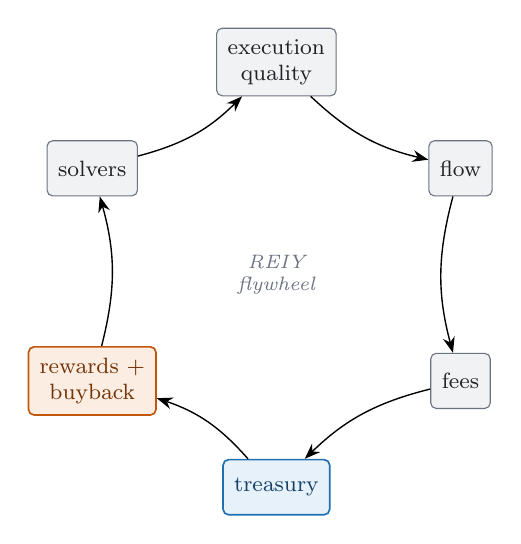
\begin{tikzpicture}[font=\footnotesize, >={Stealth[length=2mm]}]
    \def\R{2.7}
    \node[support]  (exec)  at (90:\R)   {execution\\quality};
    \node[support]  (vol)   at (30:\R)   {flow};
    \node[support]  (fees)  at (-30:\R)  {fees};
    \node[onchain]  (treas) at (-90:\R)  {treasury};
    \node[offchain] (rew)   at (-150:\R) {rewards +\\buyback};
    \node[support]  (solv)  at (150:\R)  {solvers};
    \draw[flow] (exec)  to[bend right=15] (vol);
    \draw[flow] (vol)   to[bend right=15] (fees);
    \draw[flow] (fees)  to[bend right=15] (treas);
    \draw[flow] (treas) to[bend right=15] (rew);
    \draw[flow] (rew)   to[bend right=15] (solv);
    \draw[flow] (solv)  to[bend right=15] (exec);
    \node[font=\scriptsize\itshape, cSup, align=center] at (0,0) {REIY\\flywheel};
  \end{tikzpicture}}
  \caption{The value flywheel: each stage funds the next, and deeper solver
    competition feeds back into execution quality.}
  \label{fig:flywheel}
\end{figure}

The model's sensitivities are bounded and understood. Surplus, and with it the
surplus fee, varies with market conditions and competition, which is why the base
fee exists as a stabilizer. Fees accrue in a basket of traded assets and require a
treasury policy for conversion and reserves. Reaching the self funding crossover
depends on volume growth, so until it is reached the reward pool leans on emissions
and the dilution they imply. Each of these is a governable parameter, set
conservatively at launch under a multisig and handed to REIY governance as the
network matures.

\subsection{The REIY Token}

REIY is the work and governance token of the network, with three utilities.
First, it is the solver \emph{bond}: a solver must lock REIY to compete, and the
stake is slashable, so participation carries skin in the game and a failed
settlement has a cost. Second, it is the solver \emph{reward}: solvers earn REIY
in proportion to the surplus and score they deliver, which directs emissions
toward execution quality rather than raw volume. Third, it is the \emph{governance}
right: over time REIY holders govern the protocol parameters, the supported pairs,
the treasury, and the emission schedule.

Rewards are funded in two complementary ways. Early on, a scheduled emission
bootstraps a competitive solver set before fee revenue is significant. As volume
grows, the protocol treasury, which accumulates fees in traded assets, funds REIY
buyback that replenishes the reward pool, so emissions taper while real revenue
takes over. Value therefore accrues to the token through a clear loop: usage
produces fees, fees back the rewards and buyback, and bonding locks supply as a
sink, while governance grants holders control over the parameters that set all of
these. The treasury is initially held by an \texttt{AdminCap} under a multisig,
with a transition to on chain governance as the network matures.

\subsection{Bonding and Slashing}

The bond turns the right to compete into an accountable one. To register, a solver
locks at least the minimum bond in REIY; the stake gates participation and is the
value at risk if the solver misbehaves.

The slashable event is a \emph{failure to settle}. Recall from Section~5 that an
invalid settlement cannot cause loss, because the PTB simply reverts and no escrow
moves; the only way a solver can harm the batch is to win a certificate and then
not settle it before the certificate expires, which stalls the intents it was
assigned. This failure is provable from on chain state alone: the certificate
binds the solver, the epoch, and the expiry, so an assigned round left unsettled
past expiry is unambiguous evidence of default.

Slashing is not automatic, since a contract acts only when invoked; it is
triggered by a permissionless \emph{reporter}. Any party may submit the expired,
unsettled certificate to the Contract, which verifies the default from on chain
state before acting, so a false report is impossible and enforcement never depends
on the coordinator. The reporter is paid a bounty out of the slashed bond, sized
to cover gas and leave a margin, which makes catching defaults profitable for any
watcher rather than a duty that falls to no one.

The remaining bond, after the bounty, flows to the treasury and reward pool,
redistributing the cost of griefing to the honest solvers who keep settling. A
slash takes a governable fraction of the bond and escalates with repeated defaults
until a persistently failing solver is deregistered and must re-bond. Since a
default only rolls the affected intents to the next epoch through the fallback of
Section~5.6, the bond need only make repeated griefing unprofitable, not
collateralize the full trade value.

% ================================================================
\section{Security and Properties}
% ================================================================

The design goals of Section~3.3 follow from the mechanism just described. We
summarize how each is enforced and why safety does not depend on the coordinator.

\begin{property}[Non-custodial]
User funds are never under the control of any off chain party; escrow resides
solely in the shared \texttt{Intent} object.
\end{property}
\noindent The only on chain path that releases the asset is a certified
settlement that passes every check, or a cancellation by the owner.

\begin{property}[User-protected execution]
A settled trader never receives less than the protected minimum, even after fees.
\end{property}
\noindent Two floors enforce this: the SBBO floor at admission and the per intent
protected minimum at settlement, where the fee logic additionally requires the net
after fees to stay at or above that minimum.

\begin{property}[Atomic settlement]
A batch either completes in full or reverts in full.
\end{property}
\noindent The non droppable \texttt{SettlementReceipt} forces every intent taken
in a PTB to be settled in the same PTB at its exact certified payout.

\begin{property}[Permissionless competition]
Any bonded solver can win by score alone, with no whitelist.
\end{property}
\noindent This is the direct countermeasure to the entry restriction and oligopoly
that a formal analysis identifies as the central weakness of intent markets
\cite{chitra2024analysisintentbasedmarkets}.

\begin{property}[Liveness]
Neither a silent solver nor an offline coordinator can freeze the protocol.
\end{property}
\noindent Epoch advancement and certificate reissuance are permissionless or
routine operations, so the worst a faulty Fisherman can do is delay progress.

This yields a clean separation: the Fisherman governs speed and selection, but the
contract alone governs custody and correctness. A malicious coordinator cannot
move funds, cannot admit a sub floor intent, cannot pay a trader below their
minimum, and cannot make a solver win without a signature the contract verifies.
Loss of funds is impossible without a flaw in the contract itself, which narrows
the trusted surface to the audited Move modules.

% ================================================================
\section{Conclusion}
% ================================================================

Reiy brings intent based, solver competitive execution to Sui without asking users
to trust an off chain operator with their funds. Traders escrow an intent behind
an on chain SBBO floor, permissionless solvers compete to fill it, and a
certificate signed off chain is verified on chain before any asset moves, so
settlement is atomic and the user's minimum always holds. The protocol does not
replace the venues Sui already has; it turns their fragmented liquidity into depth
a single trade can reach. By keeping custody and correctness on chain while letting
coordination and competition run off chain, Reiy aims to make best execution a
default property of trading on Sui rather than a manual effort.


\bibliographystyle{acm}
\bibliography{sigproc}

\end{document}
